\section{Personas}\label{l:personas}

\begin{table}
\begin{center}
\begin{tabular}{@{}l l}
\textbf{Projektleiter} &\\
\hline
Arthur Blozyk & Sales Information and Communication\\ 
& \emph{MAN Truck \& Bus AG}\\
Sebastian Nell & Director of USE // Connected Products\\
& \emph{Scholz \& Volkmer GmbH}\\
Tobias Rudolphi	& Lead Software Architect\\
& \emph{Zühlke Engineering GmbH}\\
\textbf{Konzept, Design} &\\
\hline
Carsten Fischer	& UX Designer \& Informationsarchitekt\\
& \emph{triplesense GmbH}\\
Eva Kümml & Senior Konzept / User Experience\\
& \emph{SinnerSchrader Deutschland GmbH}\\
Sandra-Charlotte Hildebrandt & Dipl. Designerin\\
& \emph{selbständig}\\
\textbf{Produktion} &\\
\hline
Sebastian Beyer	& Developer\\
& \emph{Scholz \& Volkmer GmbH}\\
Jan Lochner	& Dipl. Multimedia Producer\\
& \emph{selbständig}\\
\textbf{Texter} &\\
\hline
Marc Stenzel & Freier Projektleiter, Fachjournalist\\
& \emph{selbständig}\\
Torsten Schölzel & Freier Texter und Konzeptioner\\
& \emph{selbständig}\\
\textbf{Übersetzer} &\\
\hline
Jorinde Gessner	& Information Manager\\
& \emph{Ogilvy \& Mather Deutschland GmbH}\\
\textbf{Kunde} &\\
\hline
Markus Rüb & Sales Information and Communication\\
& \emph{MAN Truck \& Bus AG}
\end{tabular}
\caption{Interviewte Personen}
\label{table:interviewpartner}
\end{center}
\end{table}

Im vorigen Abschnitt wurden die Probleme geschildert, die im aktuell üblichen Projektverlauf auftreten und daraus gefolgert, was die wichtigsten Aspekte sind, die eine mögliche Lösung behandeln muss. Um den Entwurf einer Lösung im nächsten Abschnitt vorzubereiten werden in diesem Abschnitt \emph{Personas} vorgestellt, die die typischen Benutzergruppen des Systems repräsentieren und ihre Aufgaben und Erwartungen zusammen fassen. Personas sind ein wichtiger Baustein für den Entwurf eines Systems. Personas ermögliche es, Konzepte und Ideen schon während des Entwurfs zu verfizieren in dem deren Auswirkungen mit dem Nutzungsverhalten und den Erwartungen der Personas verglichen werden.

\begin{quote}
\typoquotes{\textit{Personas describe a site’s target users, giving a clear picture of how they’re likely to use the system, and what they’ll expect from it, among other
things. […] Without personas, there is no common language for talking about what users want.}} \cite[S.15 ff.]{brown2007communicating}
\end{quote}

Personas bilden nicht nur im Entwurf eine wichtige Entscheidungshilfe sondern werden auch während der Umsetzung immer wieder zu Rate gezogen, in dem neue Funktionalitäten auf deren Relevanz und mögliche Probleme für bestimmte Personas hin überprüft werden. \cite[S.38 ff.]{cohn2004user}

\subsection{Überblick}

\begin{figure}[htb]
\begin{center}
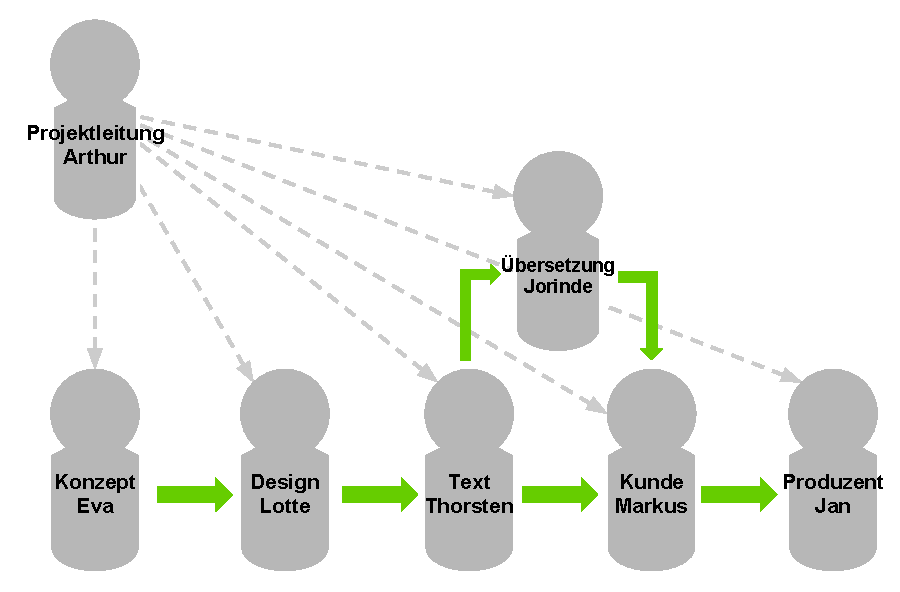
\includegraphics[width=\textwidth]{media/Uebersicht-Personas.pdf}
\caption{Übersicht über die Personas und den idealisierten Workflow}
\label{chart:uebersicht-personas}
\end{center}
\end{figure}

Die nachfolgend vorgestellten Personas basieren auf den im April 2012 geführten Interviews mit den in Tabelle~\ref{table:interviewpartner} auf Seite~\pageref{table:interviewpartner} aufgezählten Personen. Die Namen und Fotos der Personas basieren zwar auf den Interviewten Personen, dienen aber lediglich dazu, das Merken der Personas zu erleichtern. Die Auswahl der Personas orientierte sich an dem vorherrschenden Workflow innerhalb der Projekte. Wie in Abschnitt~\ref{l:problemanalyse} gezeigt wurde, gibt es in der Praxis keinen linearen Ablauf, sondern es ergeben sich vielzählige Feedback-Schleifen. Beseitigt man aber diese Feedback- und Korrektur-Schleifen kann man die beteiligten Personen in eine, in Abbildung~\ref{chart:uebersicht-personas} auf Seite~\pageref{chart:uebersicht-personas} gezeigte, lineare Reihenfolge bringen:
\begin{enumerate}\itemsep -5pt
\item Die \textbf{Konzepterin \emph{Eva}} entwickelt das Produkt, wobei sie die Rahmenbedingungen wie Aufbau, Umfang, Zielgruppe, Ansprache festlegt. 
\item Die \textbf{Designerin \emph{Lotte}} gestaltet das Produkt, wobei er bestimmt, wie Texte dargestellt werden (Satz, Länge, Schriftart, Farben, Hervorhebungen)
\item Der \textbf{Texter \emph{Thorsten}} erstellt die Texte für das Produkt in der Ausgangssprache
\item Der \textbf{Kunde \emph{Markus}} nimmt die Texte ab
\item Die \textbf{Übersetzerin \emph{Jorinde}} übersetzt die Texte
\item Der \textbf{Produzent \emph{Jan}} übernimmt die Texte in das Produkt
\end{enumerate}

Eine wichtige Rolle fehlt in dieser Aufliste: der \textbf{Projektleiter \emph{Arthur}} koordiniert den Ablauf des Projektes, hat aber keinen Einfluss den Text. Er darf jedoch als wichtiges Bindeglied zwischen allen Beteiligten  nicht fehlen.

Bei der Formulierung der Personas wurde bewusst darauf verzichtet, persönliche Daten wie Alter und Bildung zu verwenden, da diese keinen Einfluss auf den Entwurf des Systems haben. Die Personas enthalten dementsprechend nur in der linken Spalte
\begin{itemize}\itemsep -5pt
\item den wichtigsten Nutzen aus der Sicht der Person als Zitat
\item eine Beschreibung der Aufgabe der Rolle, die diese Persona repräsentiert
\item Angaben zu den Beteiligten, mit denen sich die Person im Verlauf des Projektes über Texte austauschen wird
\item die verwendeten Werkzeug zur Erfüllung der Aufgabe und die technische Erfahrung
\end{itemize}
und in der rechten Spalte
\begin{itemize}\itemsep -5pt
\item die wichtigsten Szenarios, die die Persona mit Hilfe des Systems durchführen wird
\item allgemeine Anforderungen an das System.
\end{itemize}

Nachfolgend finden sich die Steckbriefe der einzelnen Personas. 

\pagebreak

\subsection{\emph{Eva}, Konzepterin}\label{p:eva}

\begin{multicols}{2}

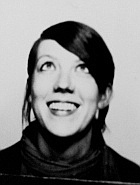
\includegraphics[width=0.5\columnwidth]{media/eva.jpg}

\typoquotes{\textit{Ich möchte, dass alle Beteiligten einen guten Überblick über das Produkt haben.}}

Eva konzipiert als Informationsarchitektin das Produkt. Dabei legt sie entsprechend der Zielsetzung fest, wie das Produkt aufgebaut ist um die Erwartungen des Nutzers zu erfüllen und ihn das gewünschten Ergebnis im Sinne des Produktes leicht erreichen zu lassen. Hierzu erstellt sie einen Überblick über das Produkt mit Hilfe von Wireframes und macht dabei Vorgaben über die Platzierung von Texten und deren Funktion.

\textbf{Abstimmung}

Eva arbeitet auf Seite der Agentur und stimmt sich mit dem Kunden~(\ref{p:markus}) und der Designerin~(\ref{p:lotte}) über das Produkt ab. Sie gibt Feedback zu den Texten des Texters~(\ref{p:thorsten}) und deren Integration in das Produkt durch den Produzenten~(\ref{p:jan}).

\textbf{Werkzeuge und technische Erfahrung}

Evas wichtigstes Werkzeug ist \emph{OmniGraffle} von \emph{Omni Group} mit dem sie die Wireframes des Produktes erstellt. Sie ist technisch versiert im Umgang mit vielfältigen Anwendung und steht neuen Werkzeugen offen gegenüber.

\columnbreak

\textbf{Szenarios}

Eva legt fest, welche Text im Produkt verwendet werden. Hierzu definiert sie die einzelnen logischen Bestandteile des Produktes (z.B. Seiten, Abschnitte) und definiert dort die einzelnen Textbausteine.

Eva legt Rahmenbedingungen für den Text fest. Zum einen bestimmt sie die Ansprache, d.h. welche Zielgruppe soll mit den Texten angesprochen werden und welches Ziel verfolgen die Nutzer. Zum anderen macht sie Vorgaben über den Aufbau einzelner Klassen von Texten wie z.B. Überschriften, Schaltflächen, Fließtext bei denen sie z.B. die Textlänge, Spaltenbreite oder Zeilenanzahl festlegt. Diese Rahmenbedingungen kann sie zu den jeweiligen Textbausteinen hinterlegen.

Eva kann sich eine Übersicht ausdrucken, die alle Bestandteile des Produktes enthält. So kann sie leicht den Überblick behalten.

\textbf{Anforderungen}

Da Eva viel Zeit mit der Definition des Produktes, der Texte und der Rahmenbedingungen verbringt, müssen diese Funktionen einfach zu bedienen sein. Sie will nie die Übersicht verlieren und leicht Elemente verändern können, da sich in der Konzeptionsphase häufig Änderungen ergeben. 

Eva hat hohe Ansprüche an die Usability und die Gestaltung des Systems.

\end{multicols}

\subsection{\emph{Lotte}, Designerin}\label{p:lotte}

\subsection{\emph{Thorsten}, Texter}\label{p:thorsten}

Copywriter sind die eigentlichen Texter, die lediglich Text erstellen, für die kein Fachwissen nötig ist, oder dieses schon vorliegt. Copywriter können Spezialwissen bezüglich SEO haben. Redakteure sind für die Gesamtheit der Texte verantwortlich und stellen sicher, dass globale Vorgaben erfüllt werden. Journalisten erstellen Texte, die auf Recherchen basieren. Diese Texte unterliegen der Sorgfaltspflicht, Quellen müssen nicht genannt werden. 

\subsection{\emph{Jorinde}, Übersetzerin}\label{p:jorinde}

\subsection{\emph{Markus}, Kunde}\label{p:markus}

\subsection{\emph{Jan}, Produzent}\label{p:jan}

\subsection{\emph{Arthur}, Projektleiter}\label{p:arthur}